\documentclass{standalone}
\usepackage{pgfplots}
\pgfplotsset{compat=1.18}

\begin{document}
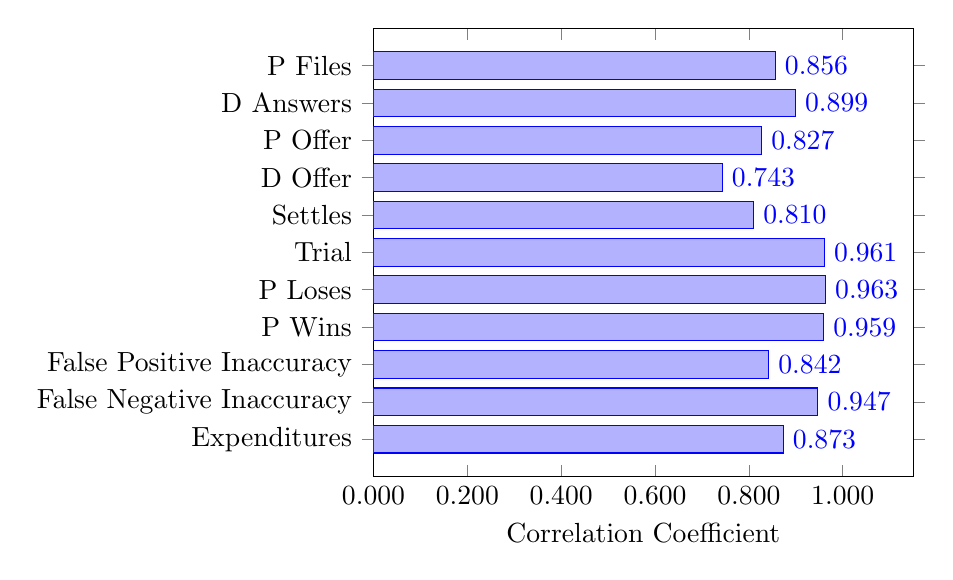
\begin{tikzpicture}
\begin{axis}[ 
xbar, xmin=0, xmax=1.15,
xlabel={Correlation Coefficient},
symbolic y coords={
    {Expenditures},
    {False Negative Inaccuracy},
    {False Positive Inaccuracy},
    {P Wins},
    {P Loses},
    {Trial},
    {Settles},
    {D Offer},
    {P Offer},
    {D Answers},
    {P Files},
    },
ytick=data,
nodes near coords,
nodes near coords align={horizontal},
/pgf/number format/.cd, fixed, fixed zerofill, precision=3,
/pgf/number format/1000 sep={},
]

\addplot coordinates {
    (0.856,{P Files}) 
    (0.899,{D Answers}) 
    (0.827,{P Offer}) 
    (0.743,{D Offer}) 
    (0.810,{Settles})
    (0.961,{Trial}) 
    (0.963,{P Loses}) 
    (0.959,{P Wins}) 
    (0.842,{False Positive Inaccuracy}) 
    (0.947,{False Negative Inaccuracy}) 
    (0.873,{Expenditures}) 
};

\end{axis}
\end{tikzpicture}
\end{document}
